\documentclass[10pt,letterpaper]{article}
\usepackage[margin=0.78in]{geometry}
\usepackage{graphicx,booktabs,tabularx,amsmath,amssymb,xcolor,hyperref,float}
\hypersetup{colorlinks=true,linkcolor=blue,urlcolor=blue}
\setlength{\parskip}{4pt}
\setlength{\parindent}{0pt}
\newcommand{\status}[1]{\textsf{#1}}
\begin{document}
{\Large\bfseries Intent2Proof: Cross-IP Contract-Abstraction Pilot}\\[3pt]
{\small Preliminary evaluation of a three-FIFO streaming subsystem and safe-shutdown requirement}\\[3pt]
\hrule
\vspace{6pt}
\textbf{Evidence status.} \textbf{Executed:} source-derived finite-state exploration and native-Z3 contract-composition/ BMC checks. \textbf{Prepared but not executed locally:} new Yosys/SymbiYosys tests on the complete multi-module RTL. The latter require an external runner. \emph{No RTL-level speedup is claimed.}

\section*{Design, property, and provenance}
The test integrates \textbf{three instances} of ZipCPU's open-source \texttt{sfifo.v} with a newly authored two-input round-robin merge and shutdown controller. The FIFO source was extracted unmodified from a previously successful pinned SBY artifact: \texttt{ZipCPU/wb2axip}, commit \texttt{2e8d3bc2d26ddc33d1881022a2a2b9d3f0c16b9b}. Its SHA-256 fingerprint is checked automatically. The same-clock subsystem accepts two input streams, merges them into a third FIFO, and drains the output under arbitrary backpressure. Three capacities (4, 8, 16) were evaluated with eight-bit payloads.

An independent external counter $P$ increments for each accepted source input and decrements for each delivered output. For the three occupancies $f_a,f_b,f_s$, the control contract requires
\begin{equation}
 P=f_a+f_b+f_s,\qquad
 \mathbf G(\mathit{reconfig\_start}\Rightarrow P=0). \label{eq:shutdown}
\end{equation}
Local handshake transitions preserve conservation because one internal transfer decrements a source FIFO and increments the sink FIFO. A deliberate negative control makes \texttt{reconfig\_start} ignore $f_s$. It can then assert during a nonempty sink buffer.

\section*{Executed local results}
\begin{center}\small
\begin{tabular}{@{}rrrrl@{}}\toprule
FIFO capacity & Reachable states & Correct model & Mutant witness & Cover conditions\\\midrule
4 & 354 & Exhaustively safe & 2 transitions & All reached\\
8 & 2,290 & Exhaustively safe & 2 transitions & All reached\\
16 & 17,106 & Exhaustively safe & 2 transitions & All reached\\\bottomrule
\end{tabular}
\end{center}
The exhaustive exploration covers every valuation of four control inputs per transition. It checks a \emph{manually transcribed, source-derived control model}, not a fully elaborated RTL system. All healthy models reached simultaneous ingress acceptance, nonempty FIFOs, shutdown with outstanding data, and safe reconfiguration. The injected defect was found for all capacities.

For each capacity, native Z3 independently checked four contract-composition obligations. The negations of (i) one-step conservation, (ii) capacity preservation, and (iii) safe shutdown were all \textsf{UNSAT}; the negative-control unsafe-shutdown condition was \textsf{SAT}. This is \textbf{12/12 expected results} at the mathematical contract level. In BMC with bound 6, all nine healthy encodings were \textsf{UNSAT} for a violation and all nine mutants were \textsf{SAT}. At bound 10 for capacity 4, all three healthy encodings timed out (\textsf{UNKNOWN}) within four seconds; all three mutants remained \textsf{SAT}.

\begin{figure}[H]\centering
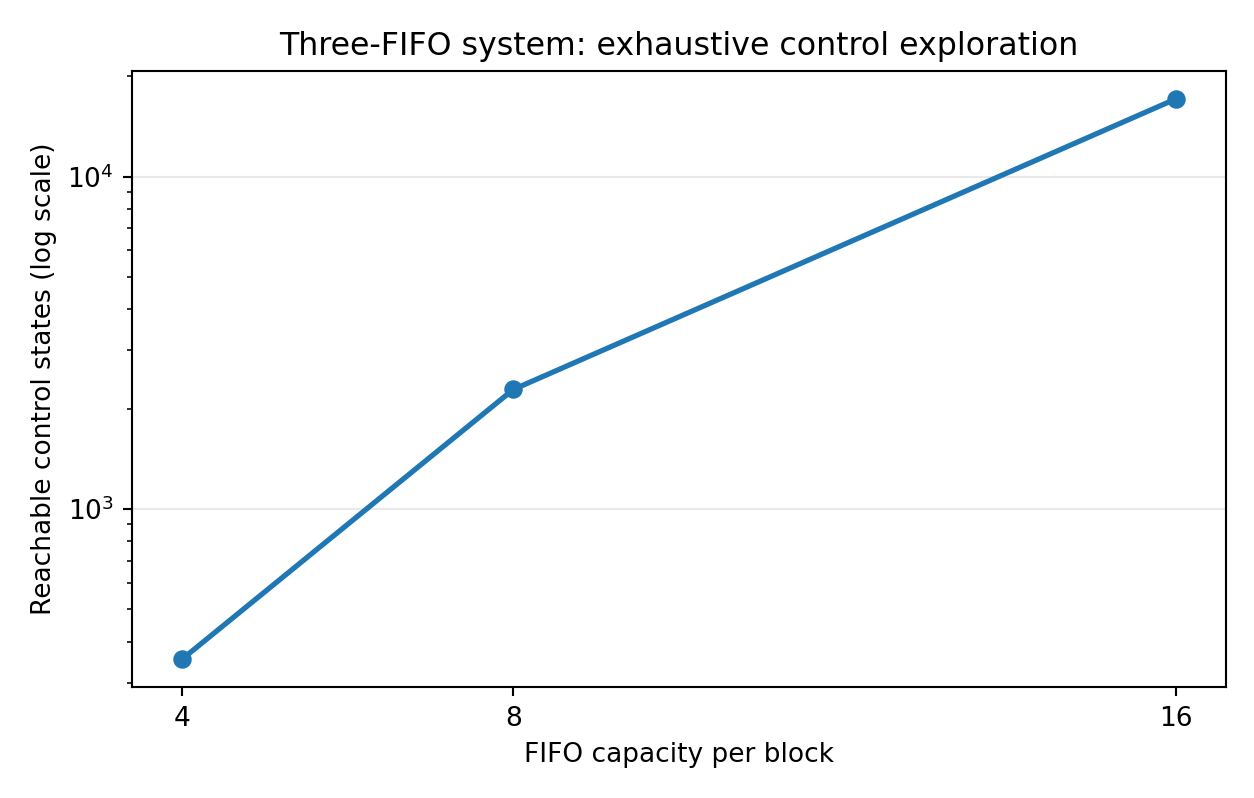
\includegraphics[width=.64\textwidth]{../figures/fig1_reachable_control_states.png}
\caption{Exhaustively explored states of the source-derived interconnected control model. Logarithmic scale. These are not Yosys-elaborated RTL state counts.}\end{figure}
\section*{Counterexample and abstraction comparison}
\begin{figure}[H]\centering
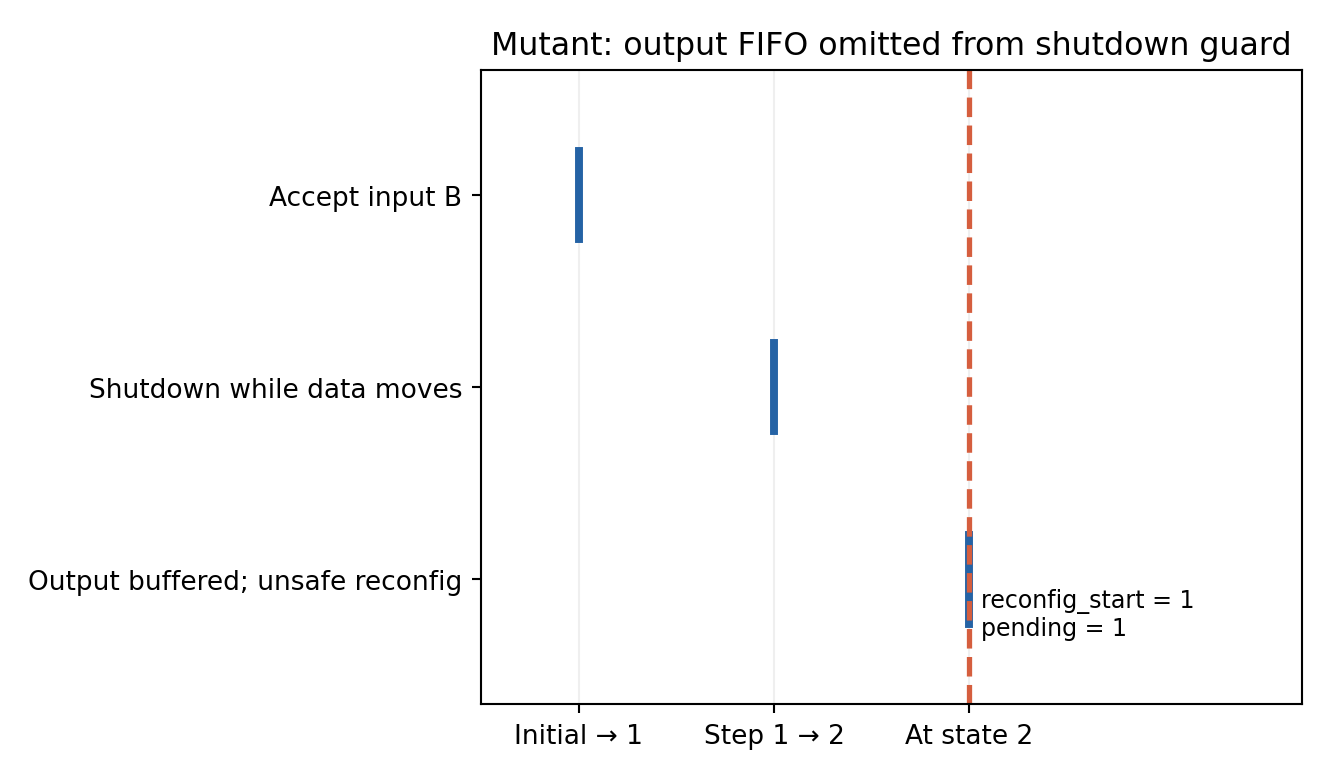
\includegraphics[width=.70\textwidth]{../figures/fig2_mutant_shutdown_counterexample.png}
\caption{Two-transition counterexample: ingress B accepts a token; shutdown occurs while the token moves to the sink FIFO; the faulty controller then starts reconfiguration with $P=1$.}\end{figure}

\begin{center}\small
\begin{tabular}{@{}rrrr@{}}\toprule
Capacity & Declared-state budget$^*$ & Standard COI bits$^*$ & Count-contract bits$^*$\\\midrule
4 & 133 & 19 & 16\\
8 & 239 & 23 & 20\\
16 & 441 & 27 & 24\\\bottomrule
\end{tabular}\\[-1pt]
{\footnotesize $^*$Computed from model/RTL declarations, not measured ABC latches.}
\end{center}

At bound 6, the median Z3 formula lengths were 29,270 bytes (augmented source-derived control), 21,845 bytes (standard COI), and 15,152 bytes (count contract). The corresponding median runtimes were 0.218, 0.204, and 0.234 seconds. Thus, the contract encoding was approximately 30.6\% smaller than standard COI \emph{without a demonstrated runtime speedup}. This is a small-model sensitivity result, not evidence of performance on actual large designs.

\begin{figure}[H]\centering
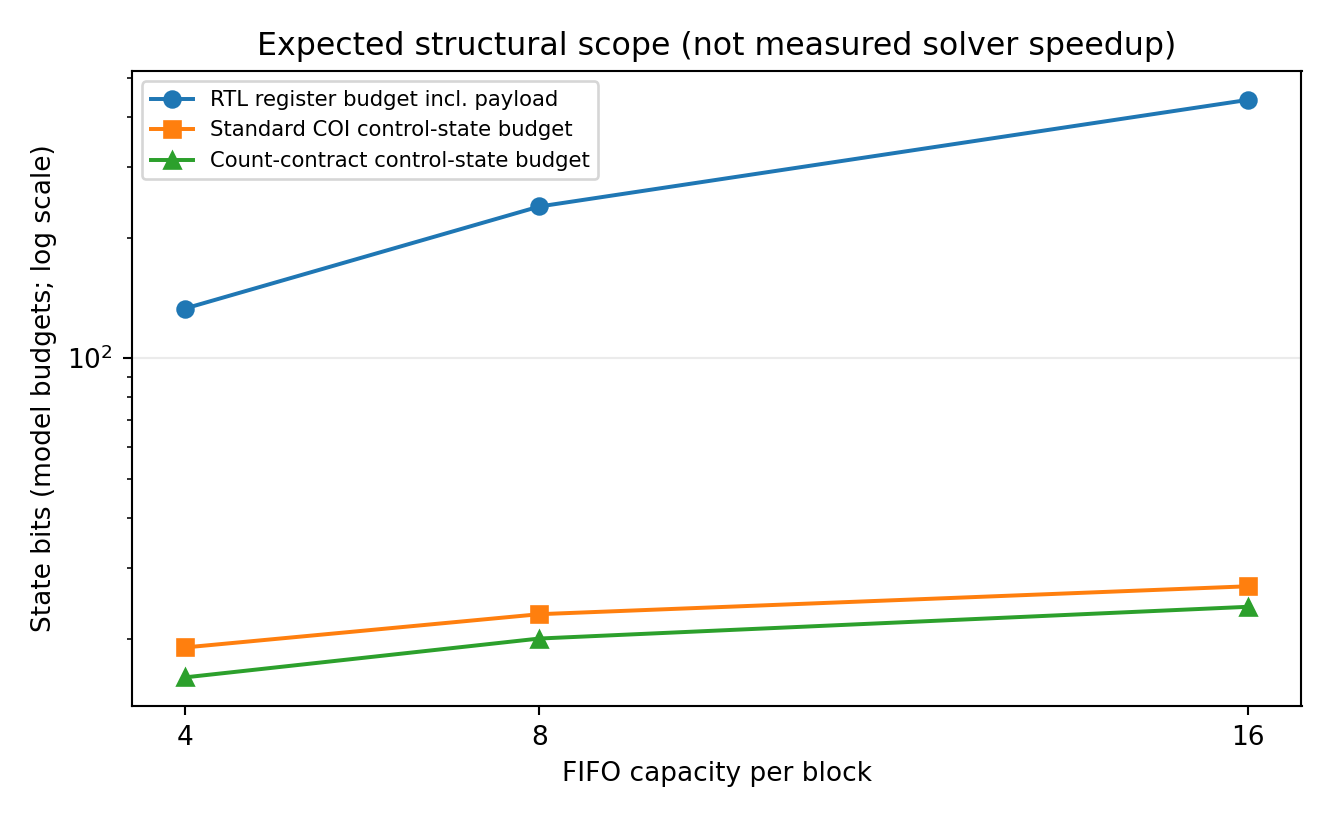
\includegraphics[width=.68\textwidth]{../figures/fig3_model_bit_budgets.png}
\caption{Illustrative structural budgets: conventional COI already strips almost all payload state. The incremental count contract eliminates three empty-flag registers across the three FIFO instances.}\end{figure}

\section*{Remaining independent RTL obligations}
The package generates 18 SBY tasks: original full RTL (3), conventional COI (3), count-contract abstraction (3), direct unit-level correspondence of the original FIFO to the count contract (3), injected defective controller (3), and non-vacuity cover checks (3). The acceptance gate requires all proofs and covers, and a waveform for each expected mutant violation; unresolved results block approval. The contract must be proved against the \emph{exact pinned source and parameter options} before substituting it into a system-level analysis. Once real-RTL SBY results are obtained, AIG latches/AND gates and the actual proof times can be compared across methods.

\textbf{Interpretation.} The executed checks support the feasibility of compositional reasoning for a meaningful cross-instance shutdown bug. They do not yet demonstrate correctness of the authored RTL integration, a sound automatically extracted abstraction, a unique algorithmic contribution, or a solver-speed advantage beyond current formal COI engines.
\end{document}
